\documentclass[runningheads]{llncs}
%
\usepackage[T1]{fontenc}
% T1 fonts will be used to generate the final print and online PDFs,
% so please use T1 fonts in your manuscript whenever possible.
% Other font encondings may result in incorrect characters.
%
\usepackage{graphicx}
% Used for displaying a sample figure. If possible, figure files should
% be included in EPS format.
%
% If you use the hyperref package, please uncomment the following two lines
% to display URLs in blue roman font according to Springer's eBook style:
\usepackage{hyperref}
\usepackage{color}
\renewcommand\UrlFont{\color{blue}\rmfamily}
\usepackage{amsmath}
\usepackage{amssymb}
\usepackage{tikz}
\usetikzlibrary{calc}

\usepackage{todonotes}


\usepackage[caption=false]{subfig}

\newcommand{\jvinline}[1]{%
  \todo[inline, color=teal, caption={}]{%
    \begin{minipage}{\linewidth}%
      #1%
    \end{minipage}%
  }%
}
% \DeclareMathOperator{\Uni}{Uni}
%
\begin{document}
%
\title{Quantum Isomorphisms of Finite Graphs -- \\A Construction from the Penrose Dodecahedron}
%
\titlerunning{Quantum Isomorphisms of Finite Graphs}
% If the paper title is too long for the running head, you can set
% an abbreviated paper title here
%
\author{
Jan Vorloeper
}
%
\authorrunning{J.\@ Vorloeper}
% First names are abbreviated in the running head.
% If there are more than two authors, 'et al.' is used.
%
\institute{
Ruhr University Bochum, Bochum, Germany \\
\email{firstname.lastname@rub.de}
}
%
\maketitle              % typeset the header of the contribution
%
\begin{abstract}
todo

\keywords{Graph Isomorphism \and Non-local Games}
\end{abstract}
%
%
%
\section{Introduction}


The recent advances in quantum information and quantum computation have profoundly transformed computational science.
There are many scientific fields that will potentially benefit from the existence of a full-scale quantum computer, 
including economics, physics (via efficient simulation of quantum systems)
and even machine learning (see e.g.~\cite{du2025quantummachinelearninghandson}).
However, the most significant and impactful application of quantum computing is in the field of
cybersecurity, as Shor's algorithm~\cite{Shor_1997} allows to break conventional asymmetric cryptography
based on prime factorization or discrete logs exponentially faster than any classical computer.
This discovery fundamentally disrupted cryptographic research, paving the way for the emergence of a new field
called post-quantum cryptography, in which new cryptographic systems are designed which conjecturally resist the
dangers of quantum algorithms.
Moreover, quantum phenomena such as superdense coding~\cite{Harrow_2004} and quantum teleportation~\cite{PhysRevLett.70.1895}
lays the groundwork for the field of quantum cryptography,
which is the study of quantum protocols resistant to eavesdropping.

A formal method to quantify these seemingly information-theoretic advantages of quantum physics
comes from the study of \emph{non-local games}.
A non-local game is an interactive cooperative game, in which the players win by fulfillling 
a given relation between the questions that are given to each player and their respective answers. 
While there is no communication allowed between the players during the game, possibly entangled quantum resources are allowed to be shared.
By leveraging this quantum advantage it is possible for the players to achieve winning
probabilities that exceed those of any classical (i.e. non-quantum) strategy.

Perhaps the best known non-local game is the magic square game
introduced in~\cite{aravind2003simpledemonstrationbellstheorem},
in which a $3 \times 3$ grid of $\pm1$ entries must be (partially) filled by the players,
such that each row multiplies to $1$ and each column multiplies to $-1$.
The first player gets asked the assignments of a specific row, while the second player
is asked about a column. The game is won if the mutual entry of the magic square is
filled with the same values by both players.
While any strategy that involves entirely filling the magic square beforehand and answering 
according to this assignment is impossible by design, it is possible to leverage the quantum resources to 
win the game with certainty.
Due to this seemingly magical phenomenon,
the magic square game is an example of what is called a \emph{pseudo-telepathic} game.

Another example of such a \emph{pseudo-telepathic} game is the graph isomorphism game,
which is parametrized by two publicly known graphs $G$ and $H$.
The referee’s questions to each player comprises of a vertex of $G$,
to which the players must answer with a vertex of $H$. 
In order to win, the nodes given as answers must fulfill the same adjacency relations in
$H$ as the nodes that are given as questions by the referee do in $G$.
While one can construct a perfect classical game strategy if and only if $G$ and $H$ are isomorphic, 
it is known that non-isomorphic graph pairs exist for which a perfect quantum strategy can be found.
Such graph pairs are said to be quantum-isomorphic.

\section{Preliminaries}
\todo{todo}

\todo[inline]{}
\subsection{Non-Local Games}

\begin{figure}
    \centering
    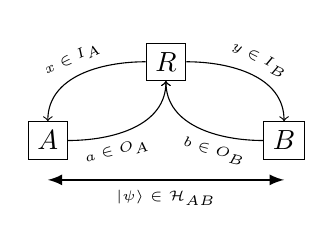
\begin{tikzpicture}
        \node[draw] at (0, 1) (r) {$R$};
        \node[draw] at (-1.5, 0) (a) {$A$};
        \node[draw] at (1.5, 0) (b) {$B$};

        \draw[->] (r) to[out=180,in=90] node[pos=0.5, sloped, above] {\tiny $x \in I_A$} (a);
        \draw[->] (a) to[out=0,in=270] node[pos=0.33, sloped, below] {\tiny $a \in O_A$} (r);
        \draw[->] (r) to[out=0,in=90] node[pos=0.5, sloped, above] {\tiny $y \in I_B$} (b);
        \draw[->] (b) to[out=180,in=270] node[pos=0.33, sloped, below] {\tiny $b \in O_B$} (r);

        \draw[thick, latex-latex] (-1.5, -0.5) -- (1.5, -0.5) node[midway, below] {\tiny $|\psi\rangle \in \mathcal{H}_{AB}$};
    \end{tikzpicture}
    \caption{Graphical illustration of how non-local games are played.}
\end{figure}

Non-local games consist of two non-communicating players $A$ and $B$, which are given 
questions $x \in I_A, y \in I_B$ by the referee, to which they must respond with an answer $a \in O_A, b \in O_B$.
The game is won if the questions and answers fulfill some predefined condition,
captured by a \emph{verification function}
\[ V: I_A \times I_B \times O_A \times O_B~\rightarrow~\{0, 1\}, \]
i.e., if $V(x, y, a, b) = 1$, the game is won.
The probability for the players to receive questions $x$ and $y$ 
are modelled via some probability distribution $\pi: I_A \times I_B \rightarrow [0, 1]$,
which, for simplicity, is generally assumed to be a uniform distribution.

The \emph{winning probability} of a non-local game $G$ using a strategy $S$ is defined as
\[ \omega_S(G) = \sum_{x,y} \pi(x, y) \sum_{a,b} V(x,y,a,b)~p(a,b~|~x,y) \]
where $p(a,b~|~x,y)$ is the probability for $A$ and $B$ to respond with $a,b$, given questions $x,y$.
Note that this is the only term that the players
have control over (by agreeing on a game strategy $S$ beforehand),
while the other terms are predetermined by the game instance that is played.

The caveat to non-local games is that the players are not allowed to communicate 
during the game, but are allowed to use (possibly entangled) quantum resources, which are distributed before the game,
to which they may apply \emph{local} changes (i.e. apply unitaries and measurements on their own share of qubits).
%
Studying non-local games is motivated by a peculiar phenomenon called \emph{quantum advantage},
describing that the pre-shared quantum resources allow to devise so called \emph{quantum strategies},
which may achieve higher winning probabilities than \emph{classical strategies},
i.e. strategies that do not utilise these quantum resources.
%
Phrased in terms of the \emph{optimal (classical / quantum) winning strategy},
\begin{align*}
    \omega^*(G) := \sup_{S \textrm{ classical}}~\omega_S(G), & & \omega_q^*(G) := \sup_{S \textrm{ quantum}} \omega_S(G),
\end{align*}
there exist non-local games $G$ for which $\omega^*(G) < \omega_q^*(G)$.
%
Furthermore, it is known that quantum strategies are \emph{non-signalling}, 
meaning that the answers of each player are statistically independent of each other,
defying intuition that some form of information exchange is happening inbetween the players during the game.









\subsubsection{Binary Constraint System Games}

\jvinline{A big class of non-local games are BCS. They are defined as ...}

\jvinline{Famous example: Magic Square}

The most prominent example of a BCS is the Magic Square Game,
which is parametrized by publicly known values $b_k \in \{ \pm 1\}$.
The magic square comprises of nine variables $X_i \in \{ \pm 1\}$ aligned in a $3 \times 3$ grid,
with the requirement that $\prod_{i \in k} X_i = b_k$.

\begin{figure}[h]
    \centering
    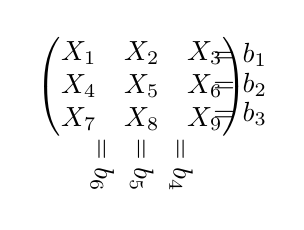
\begin{tikzpicture}
        \node[] at (0, 0) {
            $\begin{pmatrix}
                X_1 & X_2 & X_3 \\
                X_4 & X_5 & X_6 \\
                X_7 & X_8 & X_9 
            \end{pmatrix}$
            };       
        \node[] at (1.25, 0.4) {$= b_1$};
        \node[] at (1.25, 0.025) {$= b_2$};
        \node[] at (1.25, -0.35) {$= b_3$};
        \node[rotate=270] at (0.5, -1) {$= b_4$};
        \node[rotate=270] at (0, -1) {$= b_5$};
        \node[rotate=270] at (-0.5, -1) {$= b_6$};
    \end{tikzpicture}
    \caption{The Magic Square Game.}\label{fig:magic-square}
\end{figure}


The Magic Square game is now played as follows:
The referee requests a random row from player A
and a random column from player B, to which both players must respond
with a valid assignment of the involved variables.
The players win the game if and only if their assignments of the overlapping variable agree.

\begin{example}
    todo
\end{example}
\begin{figure}
    \centering
    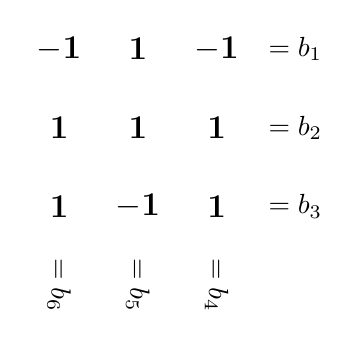
\begin{tikzpicture}
        \magicsquare{0}{0}        
        \node[] at (-1, 1)  {\large $\mathbf{-1}$};
        \node[] at (0, 1)   {\large $\mathbf{1}$};
        \node[] at (1, 1)   {\large $\mathbf{-1}$};
        \node[] at (-1, 0)  {\large $\mathbf{1}$};
        \node[] at (0, 0)   {\large $\mathbf{1}$};
        \node[] at (1, 0)   {\large $\mathbf{1}$};
        \node[] at (-1, -1) {\large $\mathbf{1}$};
        \node[] at (0, -1)  {\large $\mathbf{-1}$};
        \node[] at (1, -1)  {\large $\mathbf{1}$};

        \node[] at (2, 1) {$= b_1$};
        \node[] at (2, 0) {$= b_2$};
        \node[] at (2, -1) {$= b_3$};
        \node[rotate=270] at (1, -2) {$= b_4$};
        \node[rotate=270] at (0, -2) {$= b_5$};
        \node[rotate=270] at (-1, -2) {$= b_6$};
    \end{tikzpicture}
\end{figure}

Note that this game is parametrized by the choice
of values $b_k$, which impacts the success of classical strategies for this game.
While an all-one assignment $b_k = 1,~\forall k$ allows
the trivial strategy (always respond with $X_i = 1$) to succeed with certainty,
it is possible to choose parameters $\{b_k\}_k$, for which no optimal classical strategy exists.

\begin{lemma}
    The Magic Square game with parameters as in~\ref{} % $b_1 = b_2 = ... = b_5 = +1$, $b_6 = -1$
    has no optimal classical strategy.
\end{lemma}
\begin{proof}
    todo.
\end{proof}

Interestingly, there do exist optimal quantum strategies for the Magic Square game,
independent of the parameter choice.
\begin{lemma}
    The quantum strategy given by (todo) is an optimal strategy for the Magic Square game.
\end{lemma}    
\begin{proof}
    todo.
\end{proof}
    



% \subsubsection{Arkhipov's Construction of BCS}
% Main source~\cite{arkhipov2012extendingcharacterizingquantummagic}
% \jvinline{Intersection Graphs}
% \jvinline{
%     Main point: Non-planar graphs yield BCS with quantum advantage
% }
\todo[inline]{}
\subsubsection{The Graph Isomorphism Game}

In similar fashion, we may define the following
non-local game based on graphs.

\begin{definition}
    Let $G, H$ be graphs. The $(G, H)$-isomorphism game (or graph isomorphism game)
    is the non-local game defined by the following rules:
    \begin{itemize}
        \item Alice and Bob both receive vertices $v_A, v_B \in V(G)$
        \item They have to answer with vertices $w_A, w_B \in V(H)$
        \item The game is won if $\textrm{rel}(v_A, v_B) = \textrm{rel}(w_A, w_B)$,
        where 
        \[ \textrm{rel}:~V(\Gamma) \times V(\Gamma)~\rightarrow~\{ =, \sim, \not \sim \} \]
        denotes the adjacency relation between two vertices of some graph $\Gamma$.
    \end{itemize}
\end{definition}

Based on this, we may define the notion of a quantum isomorphism between graphs.
\begin{definition}
    Two graphs $G, H$ are said to be \emph{quantum isomorphic},
    denoted $G \cong_q H$, if there exists a perfect quantum
    strategy for the $(G, H)$-isomorphism game.
\end{definition}
\begin{remark}
    An immediate observation from those definitions is that the game can be won perfectly
    when there is a graph isomorphism $\varphi:~G \xrightarrow{\sim} H$ between both graphs,
    since a perfect (classical) strategy can be constructed by
    applying this isomorphism, i.e. by choosing $w_A = \varphi(v_A)$
    and $w_B = \varphi(v_B)$. Thus we have
    \[ G \cong H \implies G \cong_q H. \]
    Interestingly, the converse is not true.
    As we will see repeatedly, there exist pairs of graphs 
    which are quantum isomorphic yet non-isomorphic.
    These pairs of graphs are the main object of study in this work 
    and to this date, very few examples of these are known.
    Throughout this work, we will simply call such graph pairs 
    \emph{quantum isomorphic} and implictly assume
    that they are non-isomorphic, unless stated otherwise.
\end{remark}

There are many alternative definitions of graphs being quantum isomorphic
to each other, some of which are more helpful for the explicit
construction of such graph pairs.
Below we give a condition which is stated purely in graph theoretical terms.
\begin{definition}\emph{\textbf{\cite{Wang_1998}}}
Let $\mathcal{A}$ be a unital $C^*$-algebra. A \emph{magic unitary}
(or quantum permutation matrix) is a matrix $u \in M_n(\mathcal{A})$
whose entries are projections in $\mathcal{A}$, i.e.
$\forall i,j \in \{1,\dots, n\}:~u_{ij} = u_{ij}^* = u_{ij}^2$, and furthermore
\[ \forall i \in \{1,\dots, n\}:~\sum_k u_{ik} = \sum_k u_{ki} = \mathbf{1}_\mathcal{A} \]
\end{definition}
\begin{remark}
    Note that this definition generalizes the notion of
    a permutation matrix, since the definitions coincide for 
    the special case $\mathcal{A} = \mathbb{C}$
    (here the set of projections is just $\{0,1 \}$).
\end{remark}

\begin{definition}
    Let $G, H$ be graphs. $G$ and $H$ are quantum isomorphic iff
    there exists a unital $C^*$-algebra $\mathcal{A}$ and
    a magic unitary $u \in M_n(\mathcal{A})$ such that 
    \[ A_G u = u A_H, \]
    where $A_G$ and $A_H$ are the adjacency matrices of $G$ and $H$ respectively.
\end{definition}
\begin{remark}
    Continuing the previous remark, we see that the special case 
    $\mathcal{A} = \mathbb{C}$ translates to quantum isomorphisms
    being equivalent to classical isomorphisms, as the adjacency
    matrices of classically isomorphic graphs are conjugate
    under some permutation, represented by a permutation matrix.

    Moreover, the unital $C^*$-algebras appearing in our discussion about
    quantum isomorphic graph pairs will all be of the form
    $\mathcal{A} = M_n(\mathbb{C})$ for some $n > 1$.
\end{remark}

Another way of characterizing quantum isomorphisms of a fixed graph 
is done in more group-theoretic terms.
See~\cite{Musto_2018} on details about the algebraic theory
behind quantum isomorphisms.

\begin{lemma}
    \emph{\textbf{\cite[Corollary 4.15]{Musto_2018}}}
Let $G$ be a graph with no (non-classical) quantum automorphisms.
Then there is a bijection between 
\begin{itemize}
    \item Isomorphism classes of graphs $G'$ quantum-isomorphic to $G$
    \item Conjugacy classes of central type subgroups $(L, \psi) \subseteq \textrm{Aut}(G)$ with coisotropic stabilizers.
\end{itemize}
\end{lemma}
\begin{remark}
    Central type subgroups have a deep representation-theoretic description,
    which exceeds the scope of this work.
    The most prominent examples of central type subgroups appearing
    in the context of quantum isomorphisms are
    $\mathbb{Z}_n \times \mathbb{Z}_n$ for some integer
    $n \in \mathbb{N}$. 
\end{remark}
\section{Known Constructions}

\subsection{Construction of Graphs from Binary Constraint Systems}

Main source~\cite{atserias2017quantumnonsignallinggraphisomorphisms}

\jvinline{
    \begin{itemize}
        \item Give the construction via the magic square game example
        \item Show why this works
    \end{itemize}
}


\subsection{Construction of Graphs from the $E_8$ Root System}

Main source~\cite{schmidt2022quantumisomorphicstronglyregular}

\jvinline{
    A different approach, showing that quiso graphs are more general than quantum optimal BCS
}

\jvinline{
    Use the fact that $E_8$ contains 15 sets of distinct bases $e_i^{(j)}$ of $\mathbb{R}^8$,
    and use projections onto $e_0^{(j)}$ together with automorphisms mapping $e_i^{(j)}$ onto $e_{i+1}^{(j)}$
    to get a magic unitary. 
}
\section{Construction of Quantum Isomorphic Graphs from the Penrose Dodecahedron}

\subsection{Kochen-Specker Sets}

\jvinline{
    Picking up from the $E_8$ subsection right above,
    state why Kochen-Specker sets are interesting here
}
\jvinline{Another example (next to $E_8$) of a KS set is the Penrose Dodecahedron}

\subsection{The Penrose Dodecahedron}

Main sources~\cite{Vlasov2024,ZIMBA1993697}.

Let $\omega = \frac{-1 + \sqrt{3}i}{2}$ be the third root of unity over $\mathbb{C}$, satisfying $\omega^3 = 1$.
The Penrose Dodecahedron can then be defined as the following set of 40 vectors in $\mathbb{C}^4$:
\begin{align*}
    \left(1, 0, 0, 0\right) & \left(0, 1, 0, 0\right) & \left(0, 0, 1, 0\right) & \left(0, 0, 0, 1\right) \\
    \left(\right) & \left(\right) & \left(\right) & \left(\right) \\
    \left(\right) & \left(\right) & \left(\right) & \left(\right) \\
\end{align*}



% \jvinline{Give construction of it, its group structure etc.}

\question{
    Is the group we want to analyse the one called $\mathcal{W}$ in~\cite[Section 1]{Vlasov2024},
    i.e. the "transitive group of 25920 unitary projective transformations of $\mathbb{CP}^3$
    sending the configuration of 40 points to itself"?

}

\jvinline{
    Find central type subgroup with coisotropic stabilizers?
    \begin{itemize}
        \item Unlike for $E_8$, the Pauli Matrices are probably not the solution
        \item Rather, the matrices $R_k \in M_4(\mathbb{C})$, $k \in \{1, \dots, 4\}$ appearing in~\cite{Vlasov2024} seem promising:
        They fulfill the following properties: \begin{itemize}
            \item $R_k$ is unitary, i.e. $R_k R_k^\dagger = R_k^\dagger R_k = 1$
            \item $R_k^3 = 1$
            \item $R_k = R_k^T$
            \item Combining these facts, we get $R_k^2 = R_k^\dagger = \overline{R_k}$ (?)
        \end{itemize} 
        \item Furthermore, in~\cite{ZIMBA1993697} they mention two graphs $Q, Q^*$, which are similar but not isomorphic. Maybe good candidates?
    \end{itemize}
}

\jvinline{
    The approach (as for $E_8$): Look at $G$, construct magic unitary $u$, compute $A_H = u A_G u^\dagger$
    to get the pair $(G, H)$ and hope $G \not \cong H$.
}


%
% ---- Bibliography ----
%
% BibTeX users should specify bibliography style 'splncs04'.
% References will then be sorted and formatted in the correct style.
%
\bibliographystyle{splncs04}
\bibliography{biblio}
%
\end{document}


%%% Local Variables:
%%% mode: latex
%%% TeX-master: t
%%% End:
